%%%%%%%%%%%%%%%%%%%%%%%%%%%%%%%%%%%%%%%%%
% Simple Sectioned Essay Template
% LaTeX Template
%
% This template has been downloaded from:
% http://www.latextemplates.com
%
% Note:
% The \lipsum[#] commands throughout this template generate dummy text
% to fill the template out. These commands should all be removed when 
% writing essay content.
%
%%%%%%%%%%%%%%%%%%%%%%%%%%%%%%%%%%%%%%%%%

%----------------------------------------------------------------------------------------
%	PACKAGES AND OTHER DOCUMENT CONFIGURATIONS
%----------------------------------------------------------------------------------------

\documentclass[12pt]{article} % Default font size is 12pt, it can be changed here

\usepackage{geometry} % Required to change the page size to A4
\geometry{a4paper} % Set the page size to be A4 as opposed to the default US Letter

\usepackage{graphicx} % Required for including pictures

\usepackage{float} % Allows putting an [H] in \begin{figure} to specify the exact location of the figure
\usepackage{wrapfig} % Allows in-line images such as the example fish picture

\usepackage{lipsum} % Used for inserting dummy 'Lorem ipsum' text into the template

\linespread{1.2} % Line spacing

%\setlength\parindent{0pt} % Uncomment to remove all indentation from paragraphs

\graphicspath{{Pictures/}} % Specifies the directory where pictures are stored

\begin{document}
	
	%----------------------------------------------------------------------------------------
	%	TITLE PAGE
	%----------------------------------------------------------------------------------------
	
	\begin{titlepage}
		
		\newcommand{\HRule}{\rule{\linewidth}{0.5mm}} % Defines a new command for the horizontal lines, change thickness here
		
		\center % Center everything on the page
		
		\textsc{\LARGE Wits University}\\[1.5cm] % Name of your university/college
		\textsc{\Large School of Electrical and Information Engineering}\\[0.5cm] % Major heading such as course name
		\textsc{\large ELEN7046 - Software Technologies and Techniques}\\[0.5cm] % Minor heading such as course title
		
		\HRule \\[0.4cm]
		{ \huge \bfseries Group Project: Big Data Visualization}\\[0.4cm] % Title of your document
		
		\HRule \\[0.6cm]
		
		\begin{minipage}
			{0.4
				\textwidth} 
			\begin{flushleft}
				\large \emph{Authors:}\\
				Gareth \textsc{Stephenson} \\
				Matsobane \textsc{Khwinana} \\
				Sidwell \textsc{Mokhemisa} \\
				Dave \textsc{Cloete}\\
				Kyle \textsc{Trehaeven}
			\end{flushleft}
		\end{minipage}
		~ 
		\begin{minipage}
			{0.4
				\textwidth} 
			\begin{flushright}
				\large \emph{Student Number:} \\
				778919 \\
				779053  \\
				1229756 \\
				1573016 \\
				0602877N
				% Supervisor's Name
			\end{flushright}
		\end{minipage}
		\\[1cm]
		
		% Abstract
		\begin{flushleft}\large
			\textsc{Summary}\\
			
			This report presents the work done by Group 2 in response to the project brief for ELEN7046: Software Technologies and Techniques.
			
			The report will broadly focus on the following topics:
			
				\begin{itemize}
					\item The Methodology followed to execute the project;
					\item The Architecture of the solution developed for the project; and
					\item The different technologies used to deliver the solution.
				\end{itemize}
		\end{flushleft}
		{\large \today}\\[3cm] % Date, change the \today to a set date if you want to be precise
		
		%\includegraphics{Logo}\\[1cm] % Include a department/university logo - this will require the graphicx package
		
		\vfill % Fill the rest of the page with whitespace
		
	\end{titlepage}
	
	%----------------------------------------------------------------------------------------
	%	TABLE OF CONTENTS
	%----------------------------------------------------------------------------------------
	
	\tableofcontents % Include a table of contents
	
	\newpage % Begins the essay on a new page instead of on the same page as the table of contents 
	
	%----------------------------------------------------------------------------------------
	%	INTRODUCTION
	%----------------------------------------------------------------------------------------
	
	\section{Abstract} % Major section
	
	TBC
	
		%\subsection{Executive Summary} % --optional
		
		%------------------------------------------------
		
	\section{Literature Review}
		%--Where they come from
		%--What they currently do
		%--General experience
	
	%Example citation \cite{Figueredo:2009dg}.
	
	%------------------------------------------------
	
	%\subsection{Description of Acronyms} % Sub-section
	
	%IS - Information Systems \\
	
	%------------------------------------------------
	%Sample image for future reference (image to be taken out)
	%\begin{figure}[H] % Example image
	%\center{
\includegraphics[width=0.5\linewidth]{placeholder}}
	%\caption{Example image.}
	%\label{fig:speciation}
	%\end{figure}
	
	%------------------------------------------------
	%-------------
	%	MAJOR SECTION 1
	%----------------------------------------------------------------------------------------
	
	\section{Stakeholder Concerns - Big Data}
	
	%\subsection{Executive Summary} % --optional
	
	%------------------------------------------------
	
	\subsection{Collection}
	%--Where they come from
	%--What they currently do
	%--General experience
	
	
	
	%------------------------------------------------
	
	\subsection{Processing}
	


	%--Risk categories SP03
	
%	\subsubsection{Cost and Schedule}
	
	
	
	%--Earn Value Management SP01
	
	
	%--Earn Value Management SP01
	
	\subsection{Visualization}
	

	%--Summary of the above
	%--Kill project/replace project manager/continue project???
	
	%------------------------------------------------
	
	\section{Methodology}
	
	%\subsection{Explanation Summary} %--optional
	
	%------------------------------------------------
	In order for group two to successfully deliver this project, a development methodology based on IBM Rational Unified Process (RUP) was followed albeit tailored to cater for the specific needs of this project.\\
	\\
	The diagram below depicts the IBM RUP model:
	
		\begin{figure}[H] % Example image
			\center{\includegraphics[width=1.15\linewidth]{ibm1}}
			\caption{IBM Rational Unified Process (Source: RUP, Best Practices for Software Development Teams)}
			\label{fig:speciation}
		\end{figure}
		
		
	
%	\subsection{info}
	
	
	%------------------------------------------------
	
%	\subsection{Observation} % Sub-section
	
	
%	\subsubsection{Value}
	
	
	%\\subsubsection{Risk}
	%--Risk categories SP03

%	\subsubsection{Cost \& Schedule}
	

	
	%\subsection{xxx}
	
	
	%------------------------------------------------
	
	\section{Assumptions and Constraints}
	
	%\subsection{Explanation Summary} %--optional
	\subsection{Tweet Locations}
	The group encountered tweet location issues. \\
	\subsection{Pros and Cons determinations}
	Rudimentary algorithm for determining Twitter statements (tweets) that are against or for a particular candidate was adopted... \\
	%------------------------------------------------
	
	%--Earn Value Management 
	
	
	%--Summary of the above
	%--Kill project/replace project manager/continue project???

	
	
	%-----------------------------------------------
	
	\section{Success Criteria} % Major section
	
	
	\section{Architecture of the Solution}
		
	\subsection{High Level Design: Component Architecture}
	
	
		\begin{figure}[H] % Example image
			\center{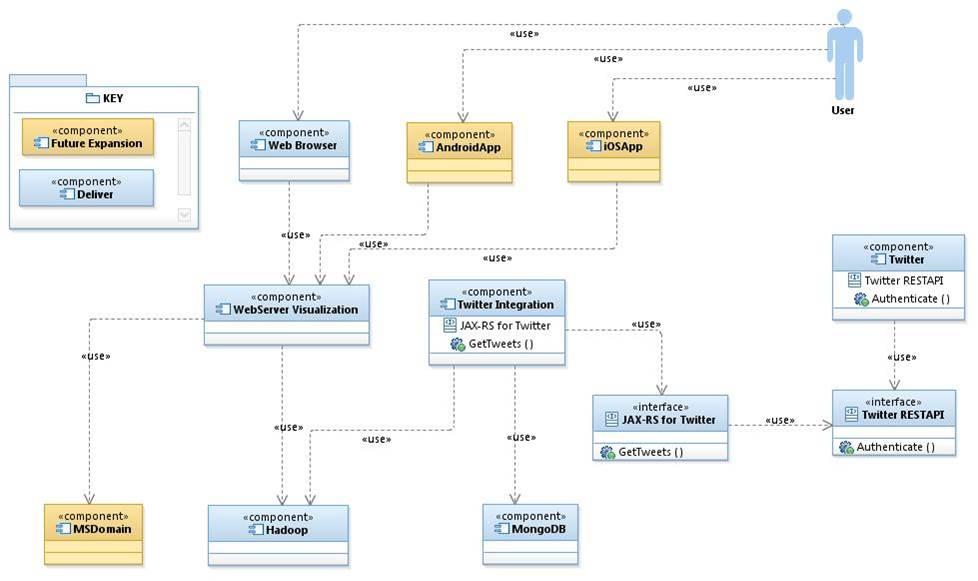
\includegraphics[width=1.15\linewidth]{HLD}}
			\caption{High Level Component Model.}
			\label{fig:speciation}
		\end{figure}
	
	\subsection{Detailed Design: Class Diagrams}
	
	\subsubsection{Data Acquisition (Batch)}
	
	\subsubsection{Data Acquisition (Streaming)}
	
	\subsubsection{Data Processing}
	
	\subsubsection{Data Visualization}
	
	\subsection{Operational Model: Infrastructure Design}
	
		\begin{figure}[H] % Example image
			\center{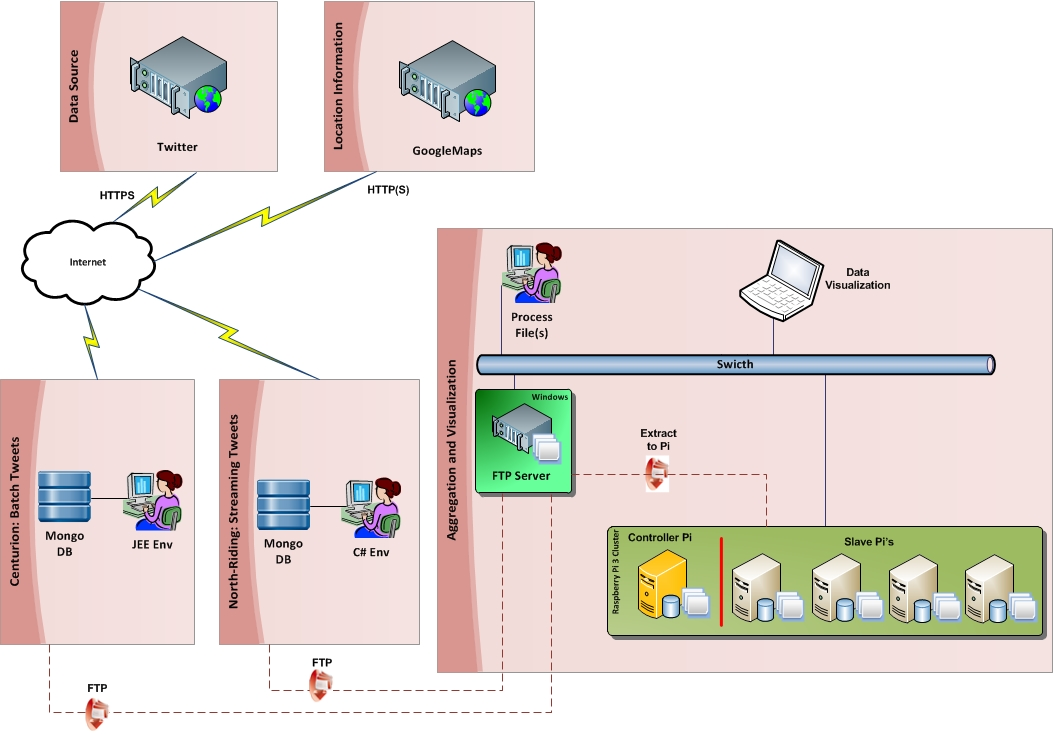
\includegraphics[width=1.15\linewidth]{ELEN7046_OM}}
			\caption{Operational Model: Phyical}
			\label{fig:speciation}
		\end{figure}
	
	%\subsection{Explanation Summary} %--optional
	
	% Risk - large project given to a small company that is running a core part of the company's systems.
	
	%------------------------------------------------
	
	%\subsubsection{Executive Summary}%--optional
	
	
	%\begin{figure}[H] % Example image
	%	\center{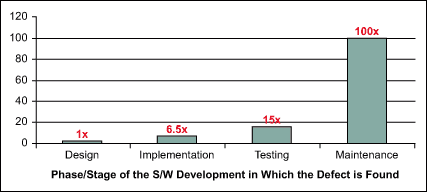
\includegraphics[width=0.55\linewidth]{IBM}}
	%	\caption{Relative Costs to Fix Software Defects (Source: IBM Systems Sciences Institute)}
	%	\label{fig:speciation}
	%\end{figure}
	
	
	
	\begin{itemize} 
		\item \textbf{Personnel Shortfall:} Inexperience in the management team is a potential risk, due to the possible oversight and inaccuracies . Leach does not have sufficient IS Management experience\textit{(pg 502 paragraph 4)}, the project may suffer if leach continues
		at his current position 
		
	\end{itemize}
	%----------------------------------------------------------------------------------------
	%	CONCLUSION
	%----------------------------------------------------------------------------------------
	
	\section{Conclusion} % Major section
	
	\subsection {Control Situation}
	
	\textit{Before we come to a conclusion and define the proposed actions we must first define the archetypical control situation. } Based on.. \\ %reference.
	
	
	\newpage
	
	%----------------------------------------------------------------------------------------
	%	BIBLIOGRAPHY
	%----------------------------------------------------------------------------------------
	
	\begin{thebibliography}{99} % Bibliography - this is intentionally simple in this template
		
		\bibitem[Van Vliet, 2008]{VV:2008dg}
		Van Vliet (2008).
		\newblock Software Engineering Principles and Practice
		
		\bibitem[Frederick P. Brooks, 1975]{VV:1975dg}
		Frederick P. Brooks (1975).
		\newblock The Mythical Man-Month
		
	\end{thebibliography}
	
	%----------------------------------------------------------------------------------------
	
\end{document}